\documentclass[10pt]{ctexart}
\usepackage{amsmath,amssymb,amsthm,amsfonts}
\usepackage[a4paper,left=2.5cm,right=2.5cm,top=2cm,bottom=2cm]{geometry}
\usepackage{graphicx,booktabs}
\usepackage{float,bm}
\usepackage{subfigure}
\author{2000012425 张弛}
\title{计算物理第二次作业}
\CTEXsetup[format={\Large\bfseries}]{section}
\newtheorem*{answer}{答}
\newtheorem*{solution}{解}
\newtheorem*{fuck}{证明}
\begin{document}
\maketitle
1.编写高斯消元法和Cholesky方法的代码,特别是求解如下线性方程组:
\begin{align}
    0.05x_1+0.07x_2+0.06x_3+0.05x_4&=0.23\notag\\
    0.07x_1+0.10x_2+0.08x_3+0.07x_4&=0.32\notag\\
    0.06x_1+0.08x_2+0.10x_3+0.09x_4&=0.33\notag\\
    0.05x_1+0.07x_2+0.09x_3+0.10x_4&=0.31.\notag
\end{align}
请将两种方法的计算结果以及Cholesky分解得到的上三角矩阵写到答案文档中。
\begin{answer}
    这次使用的是不完全支点遴选。代码见“HW2计物第一题”。两种方法计算得到的结果如下。
    \begin{table}[H]
        \centering
        \begin{tabular}{ccccc}
            \toprule
            index & 1 & 2 & 3 & 4\\
            \midrule
            GEM & 0.9999999999999328 & 1.0000000000000395 & 1.0000000000000195 & 0.9999999999999879\\
            Cholesky & 0.9999999999998956 & 1.0000000000000624 & 1.0000000000000278 & 0.9999999999999836\\
            \bottomrule
        \end{tabular}
        \caption{两种方法的计算结果}
    \end{table}
    上三角矩阵如下。
    $$
    \begin{pmatrix}
        0.22360679774997896 & 0.3130495168499706 & 0.2683281572999748 & 0.223606797749979\\
        0 & 0.04472135954999535 & -0.08944271909999287 & -3.103167691559122e-16\\
        0 & 0 & 0.14142135623730867 & 0.2121320343559652\\
        0 & 0 & 0 & 0.07071067811865184
    \end{pmatrix}$$
\end{answer}
2.对$f(x)=\cos{(x^2)},x_0=0,x_1=0.6,x_2=0.9$,采用三次样条插值,分别考虑如下两种边界条件\\
(a)$x_0=0$和$x_2=0.9$端点处的二次导数值为$0$;
\begin{solution}
    设
    $$y_0=\cos{(x_0^2)}=1,y_1=\cos{(x_1^2)}=0.935897,y_2=\cos{(x_2^2)}=0.689498.$$
    再设
    \begin{align}
        S_{01}''&=M_1\frac{x-x_0}{x_1-x_0}+M_0\frac{x_1-x}{x_1-x_0},\notag\\
        S_{12}''&=M_2\frac{x-x_1}{x_2-x_1}+M_1\frac{x_2-x}{x_2-x_1},\notag\\
        S_{01}'&=\frac{M_1}{2}\frac{(x-x_0)^2}{x_1-x_0}-\frac{M_0}{2}\frac{(x_1-x)^2}{x_1-x_0}+A_0,\notag\\
        S_{12}'&=\frac{M_2}{2}\frac{(x-x_1)^2}{x_2-x_1}-\frac{M_1}{2}\frac{(x_2-x)^2}{x_2-x_1}+A_1,\notag\\
        S_{01}&=\frac{M_1}{6}\frac{(x-x_0)^3}{x_1-x_0}-\frac{M_0}{6}\frac{(x-x_1)^3}{x_1-x_0}+A_0(x-x_0)+B_0,\notag\\
        S_{12}&=\frac{M_2}{6}\frac{(x-x_1)^3}{x_2-x_1}-\frac{M_1}{6}\frac{(x-x_2)^3}{x_2-x_1}+A_1(x-x_1)+B_1.\notag
    \end{align}
    $x_0,x_1,x_2$处的值为$y_0,y_1,y_2$,共四个方程
    \begin{align}
        \frac{M_0}{6}(x_1-x_0)^2+B_0=y_0,\notag\\
        \frac{M_1}{6}(x_1-x_0)^2+A_0(x_1-x_0)+B_0=y_1,\notag\\
        \frac{M_1}{6}(x_2-x_1)^2+B_1=y_1,\notag\\
        \frac{M_2}{6}(x_2-x_1)^2+A_1(x_2-x_1)+B_1=y_2.\notag
    \end{align}
    可以得到用$M_0,M_1,M_2$表示的$A_0,A_1,B_0,B_1$
    \begin{align}
        B_0&=y_0-\frac{M_0}{6}(x_1-x_0)^2,\notag\\
        A_0&=\frac{y_1-y_0}{x_1-x_0}-\frac{(M_1-M_0)(x_1-x_0)}{6},\notag\\
        B_1&=y_1-\frac{M_1}{6}(x_2-x_1)^2,\notag\\
        A_1&=\frac{y_2-y_1}{x_2-x_1}-\frac{(M_2-M_1)(x_2-x_1)}{6}.\notag
    \end{align}
    $x_1$处一阶导数连续
    $$\frac{M_1}{2}(x_1-x_0)+A_0=\frac{M_1}{2}(x_1-x_2)+A_1.$$
    端点二阶导数为0
    \begin{align}
        M_0&=0,\notag\\
        M_2&=0.\notag
    \end{align}
    整理得到三个关于$M_0,M_1,M_2$的方程
    \begin{align}
        0.1M_0+0.3M_1+0.05M_2&=-0.714489,\notag\\
        M_0&=0,\notag\\
        M_2&=0.\notag
    \end{align}
    解得
    \begin{align}
    M_0&=0,\notag\\
    M_1&=-2.38163,\notag\\
    M_2&=0,\notag\\
    B_0&=1,\notag\\
    A_0&=0.131324,\notag\\
    B_1&=0.971621,\notag\\
    A_1&=-0.940410.\notag
    \end{align}
    得到三次样条插值
    \begin{align}
    S_{01}&=-0.661564x^3+0.131324 x+1,\notag\\
    S_{12}&=1.32313x^3-3.57245 x^2+2.27479 x+0.571307 .\notag
    \end{align}
\end{solution}
(b)利用$f(x)$得到$x_0=0$和$x_2=0.9$端点处的一次导数值。
\begin{solution}
    要求端点一阶导数满足
    $$S_{01}'(x_0)=0,S_{12}'(x_2)=-1.30372.$$
    也即
    \begin{align}
        -\frac{M_0}{2}(x_1-x_0)+A_0&=0,\notag\\
        \frac{M_2}{2}(x_2-x_1)+A_1&=-1.30372.\notag
    \end{align}
    所以关于$M_0,M_1,M_2$的三个方程是
    \begin{align}
        0.1M_0+0.3M_1+0.05M_2&=-0.714489,\notag\\
        0.2M_0+0.1M_1=-0.106839,\notag\\
        0.05M_1+0.1M_2=-0.482392\notag
    \end{align}
    解得
    \begin{align}
        M_0=0.398857,\notag\\
        M_1=-1.866104,\notag\\
        M_2=-3.890868,\notag\\
        B_0=0.976069,\notag\\
        A_0=0.119657,\notag\\
        B_1=0.963888,\notag\\
        A_1=-0.72009.\notag
    \end{align}
    得到三次样条插值
    \begin{align}
        S_{01}&=-0.629156 x^3+0.199429 x^2+ 3.72797\times 10^{-7}x +1,\notag\\
        S_{12}&=-1.12487 x^3+1.09171 x^2 -0.53537 x+1.10707.\notag
    \end{align}
\end{solution}
3.在区间$[1,2]$内利用0-4阶和0-6阶Chebyshev多项式展开$\log_2(x)$,对结果和误差作图并分析。
\begin{solution}
    换元$x'=2x-3$,有
    $$f(x')=\log_2\left(\frac{x'}{2}+\frac{3}{2}\right).$$
    最佳平方近似有
    $$c_k=\frac{2-\delta_{0k}}{\pi}\int_{-1}^{1}\frac{T_k(x)f(x)}{\sqrt{1-x^2}}dx.$$
    另一种近似方法
    $$c_{N,m}=\frac{2-\delta_{0m}}{N}\sum\limits_{k=0}^{N-1}T_m(x_{N,k})f(x_{N,k}).$$
    数值计算无原则困难,没有必要展示代码,得到系数如下。
    \begin{table}[H]
        \centering
        \begin{tabular}{cccccc}
            \toprule
            index & 0 & 1 & 2 & 3 & 4\\
            \midrule
            最佳平方近似 & 0.543107 & 0.495055 & -0.042469 & 0.00485768 & -0.000625085\\
            另一种近似 & 0.543107 & 0.495055 & -0.0424687 & 0.00485588 & -0.000612818\\
            \bottomrule
        \end{tabular}
        \caption{4阶展开系数}
        \ \\
        \begin{tabular}{cccccccc}
        \toprule
        index & 0 & 1 & 2 & 3 & 4 & 5 & 6\\
        \midrule
        最佳平方近似 & 0.543107 & 0.495055 & -0.042469 & 0.00485768 & -0.000625085 & 0.0000857981 & -0.0000122672\\
        另一种近似 & 0.543107 & 0.495055 & -0.042469 &0.00485768 &-0.000625079 &0.0000857568 &-0.0000119964\\
        \bottomrule
        \end{tabular}
        \caption{6阶展开系数}
    \end{table}
    在绘图时换元换回来。也即
    $$g(x)=\sum\limits_{k=0}^{N-1}c_kT_{k}(2x-3).$$
    对于四阶展开式得到下图。不完整的绘图代码见“HW2计物第三题”。其中"func1"为4阶最佳平方近似,“func2”为4阶另一种近似,“func3”为6阶最佳平方近似,
    “func4”为6阶另一种近似。
    \begin{figure}[H]
        \centering
        \begin{minipage}{0.45\linewidth}
            \centering
            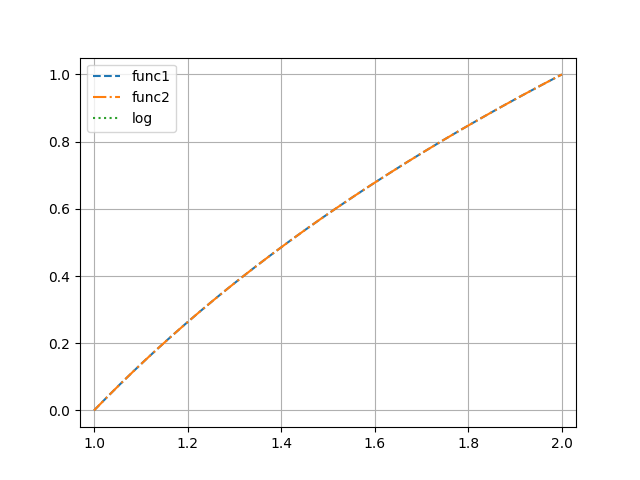
\includegraphics[width=8cm]{4.png}
            \caption{4阶}
        \end{minipage}
        \qquad
        \begin{minipage}{0.45\linewidth}
            \centering
            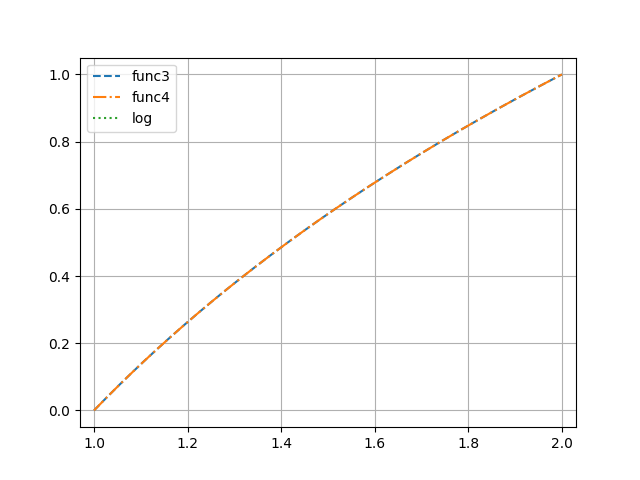
\includegraphics[width=8cm]{6.png}
            \caption{6阶}
        \end{minipage}
    \end{figure}
    从图上看来,曲线完全重合,误差极小。下面把它们与原函数的差值分别画出来。
    \begin{figure}[H]
        \centering
        \begin{minipage}{0.45\linewidth}
            \centering
            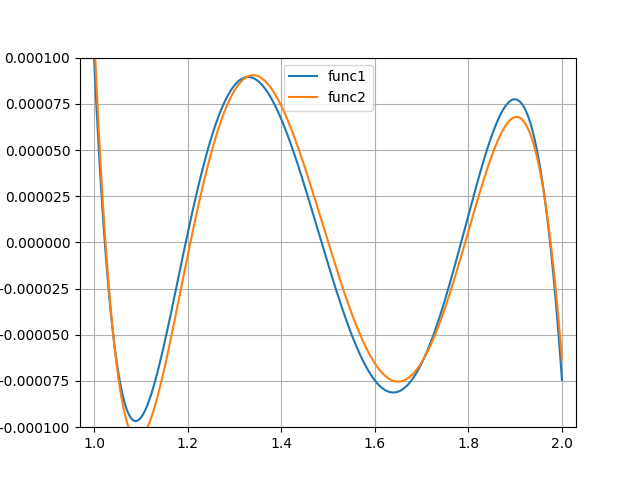
\includegraphics[width=8cm]{err4.png}
            \caption{4阶误差$\left [func(x)-\log_{2}{x}\right ]$}
        \end{minipage}
        \qquad
        \begin{minipage}{0.45\linewidth}
            \centering
            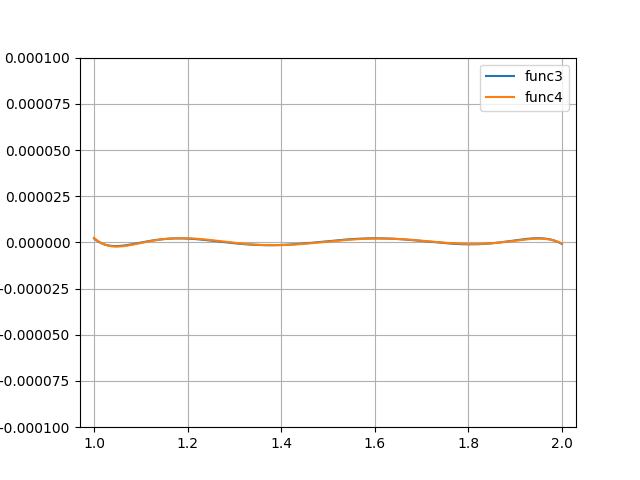
\includegraphics[width=8cm]{err6.png}
            \caption{6阶误差$\left [func(x)-\log_{2}{x}\right ]$}
        \end{minipage}
    \end{figure}
    可以看出同一阶的两种近似方法的误差很近,而6阶比4阶的误差要小很多。
\end{solution}
\textbf{4.Runge效应}\ 考虑Runge函数$f(x)=1/(1+25x^2)$在区间$[-1,+1]$上的行为。本题中将分别利用等间距的多项式内插、
Chebyshev内插以及三次样条函数来近似$f(x)$的数值。

(a)考虑$x\in[-1,+1]$之间21个均匀分布的节点(包括端点,相隔0.1一个点)的20阶多项式$P_{20}(x)$之内插(你可以利用各种方法,例如拉格朗日内插、牛顿内插或者Neville方法)。给出一个表分别列出$x,f(x),P_{20}(x)$以及两者差的绝对值。为了看出两者的区别请在这21个
点分成的每个小段的中点也取一个数据点并一起列出(因此共有41个点),同时画图显示之。
\begin{answer}
    考虑使用Neville方法,借助程序“HW2计物第四题a”得到需要的一切。
    \begin{table}[H]
        \centering
        \begin{tabular}{cccccccc}
            \toprule
            x & -1.00 & -0.95 & -0.90 & -0.85 & -0.80 & -0.75 & -0.70 \\
            \midrule
            f(x) & 3.846e-02 & 4.244e-02 & 4.706e-02 & 5.246e-02 & 5.882e-02 & 6.639e-02 & 7.547e-02\\
            $P_{20}(x)$ & 3.846e-02 & -3.995e+01 & 4.706e-02 & 3.455e+00 & 5.882e-02 & -4.471e-01 & 7.547e-02\\
            $\lvert f(x)-P_{20}(x)\rvert$ & 1.388e-17 & 3.999e+01 & 6.939e-18 & 3.402e+00 & 9.714e-17 & 5.134e-01 & 0.000e+00\\
            \bottomrule
            \toprule
            x & -0.65 & -0.60 & -0.55 & -0.50 & -0.45 & -0.40 & -0.35 \\
            \midrule
            f(x) & 8.649e-02 & 1.000e-01 & 1.168e-01 & 1.379e-01 & 1.649e-01 & 2.000e-01 & 2.462e-01 \\
            $P_{20}(x)$ & 2.024e-01 & 1.000e-01 & 8.066e-02 & 1.379e-01 & 1.798e-01 & 2.000e-01 & 2.384e-01  \\
            $\lvert f(x)-P_{20}(x)\rvert$ & 5.551e-17 & 1.159e-01 & 3.613e-02 & 1.110e-16 & 1.481e-02 & 5.551e-17 & 7.708e-03 \\
            \bottomrule
            \toprule
            x & -0.30 & -0.25 & -0.20 & -0.15 & -0.10 & -0.05 & 0.00 \\
            \midrule
            f(x) &  3.077e-01 & 3.902e-01  & 5.000e-01 & 6.400e-01 & 8.000e-01 & 9.412e-01 & 1.000e+00 \\
            $P_{20}(x)$ &  3.077e-01 & 3.951e-01& 5.000e-01 & 6.368e-01 & 8.000e-01 & 9.425e-01 & 1.000e+00  \\
            $\lvert f(x)-P_{20}(x)\rvert$ & 2.220e-16 & 4.849e-03& 4.441e-16 &  3.245e-03 & 2.220e-16 & 1.314e-03 & 6.661e-16\\
            \bottomrule
            \toprule
            x & 0.05 & 0.10 & 0.15 & 0.20 & 0.25 & 0.30 & 0.35 \\
            \midrule
            f(x) &  9.412e-01 & 8.000e-01  & 6.400e-01 & 5.000e-01 & 3.902e-01 & 3.077e-01 & 2.462e-01 \\
            $P_{20}(x)$ &  9.425e-01 & 8.000e-01& 6.368e-01 & 5.000e-01 & 3.951e-01 & 3.077e-01 & 2.384e-01 \\
            $\lvert f(x)-P_{20}(x)\rvert$ & 1.314e-03 & 1.443e-15& 3.245e-03 & 1.110e-16 & 4.849e-03 & 3.886e-16 &  7.708e-03\\
            \bottomrule
            \toprule
            x & 0.40 & 0.45 & 0.50 & 0.55 & 0.60 & 0.65 & 0.70 \\
            \midrule
            f(x) &  2.000e-01 & 1.649e-01  & 1.379e-01& 1.168e-01  &  1.000e-01 &8.649e-02 &7.547e-02\\
            $P_{20}(x)$ &  2.000e-01 & 1.798e-01 & 1.379e-01 & 8.066e-02& 1.000e-01 & 2.024e-01& 7.547e-02 \\
            $\lvert f(x)-P_{20}(x)\rvert$ & 8.327e-17& 1.481e-02& 1.943e-16 & 3.613e-02& 8.327e-17 & 1.159e-01 & 5.551e-17\\
            \bottomrule
            \toprule
            x & 0.75 & 0.80 & 0.85 & 0.90 & 0.95 & 1.00\\
            \midrule
            f(x) &  6.639e-02 & 5.882e-02  & 5.246e-02&  4.706e-02  &  4.244e-02 &3.846e-02&\\
            $P_{20}(x)$ &  -4.471e-01 & 5.882e-02 & 3.455e+00&4.706e-02& -3.995e+01 & 3.846e-02 &\\
            $\lvert f(x)-P_{20}(x)\rvert$ & 5.134e-01&  1.318e-16& 3.402e+00 & 2.776e-17& 3.999e+01 & 1.665e-16&\\
            \bottomrule
        \end{tabular}
        \caption{Neville方法的内插结果与误差}
    \end{table}
    \begin{figure}[H]
        \centering
        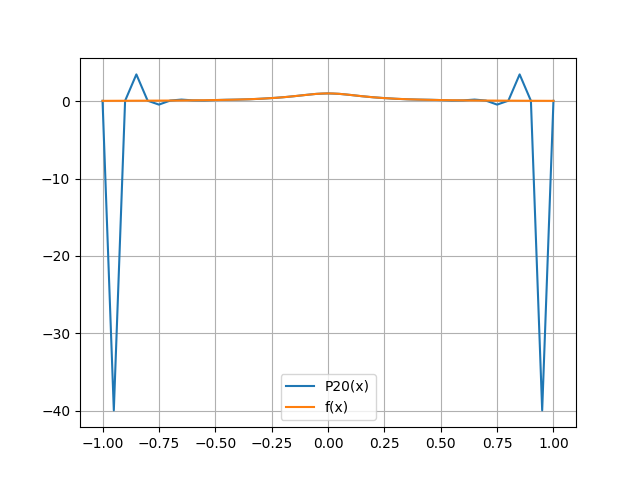
\includegraphics[width=9cm]{Neville.png}
        \caption{Neville方法的内插结果}
    \end{figure}
\end{answer}
(b)现在选取$n=20$并将上问中均匀分布的节点换为标准的Chebyshev节点:
$$x_k=\cos{\left(\frac{\pi(k+1/2)}{20}\right)},k=0,1,\cdots,19.$$
然后构造$f(x)$在$[-1,+1]$上的近似式,
$$f(x)\approx C(x)\equiv-\frac{c_0}{2}+\sum\limits_{k=0}^{19}c_kT_k(x).$$
其中在各个Chebyshev的节点处我们要求它严格等于$f(x)$。同样列出上问的表并画图,与上问结果比较。
\begin{answer}
    似乎不能使用最佳平方近似,相关数值计算借助程序“HW2计物第四题b”。展开系数如下
    \begin{table}[H]
        \centering
        \begin{tabular}{ccccccccccc}
            \toprule
            index & 0 & 1 & 2 & 3 & 4 & 5 & 6 & 7\\
            \midrule
            c & 1.960e-01 & -6.939e-19 & -2.633e-01 & 1.041e-17 & 1.768e-01 & -1.166e-16 & -1.186e-01 & 1.457e-16\\
            \bottomrule
            \toprule
            index & 8 & 9 & 10 & 11 & 12 & 13 & 14 & 15\\
            \midrule
            c & 7.932e-02 & -2.082e-18 & -5.275e-02 & -5.135e-17 & 3.463e-02 & -3.678e-17 & -2.205e-02 & 1.972e-16\\
            \bottomrule
            \toprule
            index & 16 & 17 & 18 & 19 & & & &\\
            \midrule
            c & 1.299e-02 &-3.157e-17 &-6.014e-03 &-4.766e-17\\
            \bottomrule
        \end{tabular}
        \caption{Chebyshev展开系数}
    \end{table}
    决定还是取上题41个点,得到如下结果。
    \begin{table}[H]
        \centering
        \begin{tabular}{cccccccc}
            \toprule
            x & -1.00 & -0.95 & -0.90 & -0.85 & -0.80 & -0.75 & -0.70 \\
            \midrule
            f(x) & 3.846e-02 & 4.244e-02 & 4.706e-02 & 5.246e-02 & 5.882e-02 & 6.639e-02 & 7.547e-02\\
            $P_{20}(x)$ & 3.702e-02 &  4.085e-02 & 4.869e-02 & 5.226e-02 & 5.671e-02 & 6.717e-02 & 7.825e-02\\
            $\lvert f(x)-P_{20}(x)\rvert$ & 1.446e-03 & 1.592e-03 & 1.626e-03 &  1.981e-04 & 2.110e-03 &7.792e-04 & 2.780e-03\\
            \bottomrule
            \toprule
            x & -0.65 & -0.60 & -0.55 & -0.50 & -0.45 & -0.40 & -0.35 \\
            \midrule
            f(x) & 8.649e-02 & 1.000e-01 & 1.168e-01 & 1.379e-01 & 1.649e-01 & 2.000e-01 & 2.462e-01 \\
            $P_{20}(x)$ & 8.653e-02 & 9.641e-02 & 1.141e-01 & 1.405e-01 & 1.711e-01 & 2.028e-01 & 2.402e-01  \\
            $\lvert f(x)-P_{20}(x)\rvert$ & 4.721e-05 & 3.587e-03 &  2.663e-03 & 2.592e-03 & 6.176e-03 &2.763e-03 & 5.979e-03 \\
            \bottomrule
            \toprule
            x & -0.30 & -0.25 & -0.20 & -0.15 & -0.10 & -0.05 & 0.00 \\
            \midrule
            f(x) &  3.077e-01 & 3.902e-01  & 5.000e-01 & 6.400e-01 & 8.000e-01 & 9.412e-01 & 1.000e+00 \\
            $P_{20}(x)$ &  2.963e-01 & 3.853e-01& 5.119e-01 & 6.639e-01 & 8.126e-01 & 9.221e-01 &  9.624e-01  \\
            $\lvert f(x)-P_{20}(x)\rvert$ & 1.136e-02 & 4.909e-03& 1.189e-02 &  2.385e-02 & 1.261e-02 & 1.910e-02 & 3.759e-02\\
            \bottomrule
            \toprule
            x & 0.05 & 0.10 & 0.15 & 0.20 & 0.25 & 0.30 & 0.35 \\
            \midrule
            f(x) &  9.412e-01 & 8.000e-01  & 6.400e-01 & 5.000e-01 & 3.902e-01 & 3.077e-01 & 2.462e-01 \\
            $P_{20}(x)$ &  9.221e-01 & 8.126e-01& 6.639e-01 & 5.119e-01 & 3.853e-01 & 2.963e-01 & 2.402e-01\\
            $\lvert f(x)-P_{20}(x)\rvert$ & 1.910e-02 & 1.261e-02& 2.385e-02 & 1.189e-02 & 4.909e-03 & 1.136e-02 & 5.979e-03\\
            \bottomrule
            \toprule
            x & 0.40 & 0.45 & 0.50 & 0.55 & 0.60 & 0.65 & 0.70 \\
            \midrule
            f(x) &  2.000e-01 & 1.649e-01  & 1.379e-01& 1.168e-01  &  1.000e-01 &8.649e-02 &7.547e-02\\
            $P_{20}(x)$ &  2.028e-01 & 1.711e-01 & 1.405e-01 & 1.141e-01& 9.641e-02 & 8.653e-02& 7.825e-02\\
            $\lvert f(x)-P_{20}(x)\rvert$ & 2.763e-03& 6.176e-03& 2.592e-03 & 2.663e-03& 3.587e-03 & 4.721e-05 & 2.780e-03\\
            \bottomrule
        \end{tabular}
        \caption{Chebyshev内插结果与误差}
    \end{table}
    \begin{table}
        \centering
        \begin{tabular}{cccccccc}
            \toprule
            x & 0.75 & 0.80 & 0.85 & 0.90 & 0.95 & 1.00\\
            \midrule
            f(x) &  6.639e-02 & 5.882e-02  & 5.246e-02&  4.706e-02  &  4.244e-02 &3.846e-02&\\
            $P_{20}(x)$ &  6.717e-02 & 5.671e-02 & 5.226e-02&4.869e-02 & 4.085e-02 & 3.702e-02 &\\
            $\lvert f(x)-P_{20}(x)\rvert$ & 7.792e-04& 2.110e-03& 1.981e-04 & 1.626e-03& 1.592e-03 & 1.446e-03&\\
            \bottomrule
        \end{tabular}
        \caption{Chebyshev内插结果与误差(续表)}
    \end{table}
    两个函数的图像和误差如下。
    \begin{figure}[H]
        \centering
        \begin{minipage}{0.45\linewidth}
            \centering
            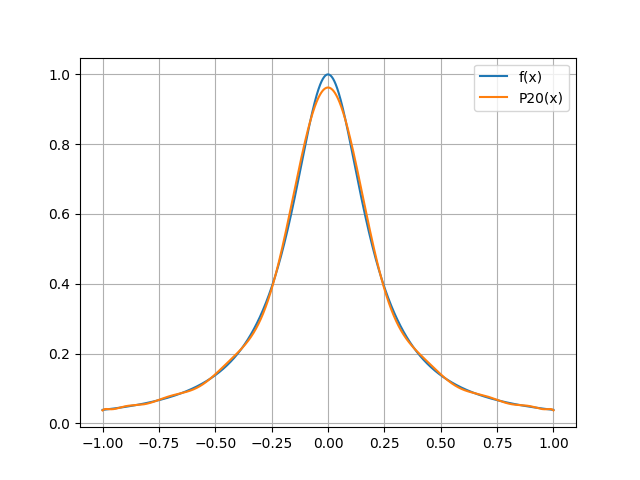
\includegraphics[width=8cm]{Chebyshev.png}
            \caption{Chebyshev内插图像}
        \end{minipage}
        \qquad
        \begin{minipage}{0.45\linewidth}
            \centering
            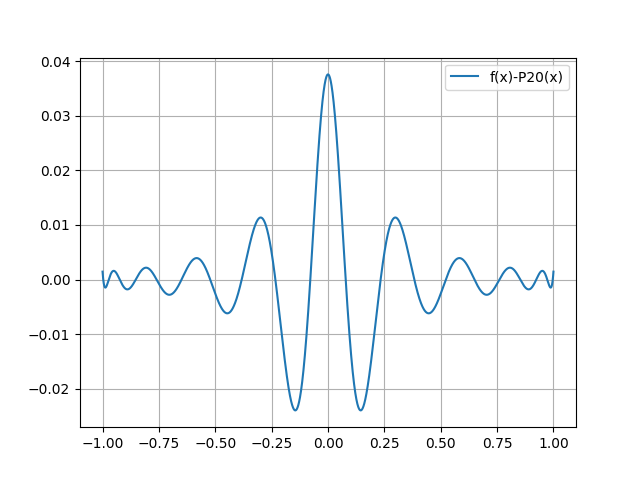
\includegraphics[width=8cm]{errChebyshev.png}
            \caption{误差$\left [f(x)-P20(x)\right ]$}
        \end{minipage}
    \end{figure}
    可以看出Chebyshev比多项式内插有更强的稳定性,节点之外没有出现离谱的偏离。
\end{answer}
(c)仍然考虑第一问中均匀分布的21个节点的内插。但这次利用21点的三次样条函数。重复上面的列表、画图并比较。
\begin{answer}
    决定使用$f(x)$的一阶导作为边界条件。设
    \begin{align}
        S_{m,m+1}''&=\frac{M_{m+1}(x-x_m)}{x_{m+1}-x_m}+\frac{M_{m}(x_{m+1}-x)}{x_{m+1}-x_m},\notag\\
        S_{m,m+1}'&=\frac{M_{m+1}}{2}\frac{(x-x_m)^2}{x_{m+1}-x_m}-\frac{M_{m}}{2}\frac{(x_{m+1}-x)^2}{x_{m+1}-x_{m}}+A_m,\notag\\
        S_{m,m+1}&=\frac{M_{m+1}}{6}\frac{(x-x_m)^3}{x_{m+1}-x_m}-\frac{M_{m}}{6}\frac{(x-x_{m+1})^3}{x_{m+1}-x_{m}}+A_m(x-x_m)+B_m.\notag
    \end{align}
    使用每段两端的节点值得到
    \begin{align}
        A_m&=\frac{y_{m+1}-y_m}{x_{m+1}-x_{m}}-\frac{M_{m+1}-M_{m}}{6}(x_{m+1}-x_{m}),\notag\\
        B_m&=y_m-\frac{M_{m}}{6}(x_{m+1}-x_m)^2.\notag
    \end{align}
    每段的端点处一阶导连续,得到
    $$\frac{x_{m+2}-x_{m+1}}{6}M_{m+2}+\frac{x_{m+2}-x_m}{3}M_{m+1}+\frac{x_{m+1}-x_m}{6}M_m=\frac{y_{m+2}-y_{m+1}}{x_{m+2}-x_{m+1}}-\frac{y_{m+1}-y_m}{x_{m+1}-x_m},m=0,\cdots,19.$$
    端点给定一阶导数,得到
    \begin{align}
        \frac{x_1-x_0}{3}M_0+\frac{x_1-x_0}{6}M_1&=-f'(x_0)+\frac{y_1-y_0}{x_1-x_0},\notag\\
        \frac{x_{21}-x_{20}}{6}M_{20}+\frac{x_{21}-x_{20}}{3}M_{21}&=f'(x_{20})-\frac{y_{21}-y_{20}}{x_{21}-x_{20}}.\notag
    \end{align}
    借由程序“HW2计物第四题c”解出线性方程组,得到20个三次样条的系数如下。
    \begin{table}[H]
        \centering
        \begin{tabular}{ccccccccc}
            \toprule
            index & 0 & 1 & 2 & 3 & 4 & 5 & 6 & 7\\
            \midrule
            M & 2.072e-01 & 3.060e-01 & 4.692e-01 & 7.474e-01 & 1.269e+00 & 2.217e+00 & 4.344e+00 & 7.781e+00 \\
            A & 8.433e-02 & 1.149e-01 & 1.618e-01 & 2.366e-01 & 3.635e-01 & 5.852e-01 & 1.020e+00 & 1.798e+00 \\
            B & 3.812e-02 & 4.655e-02 & 5.804e-02 & 7.423e-02 & 9.788e-02 & 1.342e-01 & 1.928e-01 & 2.947e-01 \\
            \bottomrule
            \toprule
            index & 8 & 9 & 10 & 11 & 12 & 13 & 14 & 15\\
            \midrule
            M & 1.530e+01 & -4.372e+00 & -5.781e+01 & -4.372e+00 & 1.530e+01 & 7.781e+00 & 4.344e+00 & 2.217e+00\\
            A & 3.328e+00 & 2.891e+00 & -2.891e+00 & -3.328e+00 & -1.798e+00 & -1.020e+00 & -5.852e-01 & -3.635e-01\\
            B & 4.745e-01 & 8.073e-01 & 1.096e+00 & 8.073e-01 & 4.745e-01 & 2.947e-01 & 1.928e-01 & 1.342e-01\\
            \bottomrule
            \toprule
            index & 16 & 17 & 18 & 19 & 20 & 21 &  &  \\
            \midrule
            M & 1.270e+00 & 7.443e-01 & 4.809e-01 & 2.620e-01 & 3.714e-01 & -4.662e-01 & & \\
            A & -2.365e-01 & -1.621e-01 & -1.140e-01 & -8.780e-02 & -5.066e-02 & & & \\
            B & 9.788e-02 & 7.423e-02 & 5.802e-02 & 4.662e-02 & 3.784e-02 & & &\\
            \bottomrule
        \end{tabular}
        \caption{三次样条系数}
    \end{table}
    上面41个点处的内插结果与误差如下。
    \begin{table}[H]
        \centering
        \begin{tabular}{cccccccc}
            \toprule
            x & -1.00 & -0.95 & -0.90 & -0.85 & -0.80 & -0.75 & -0.70 \\
            \midrule
            f(x) & 3.846e-02 & 4.244e-02 & 4.706e-02 & 5.246e-02 & 5.882e-02 & 6.639e-02 & 7.547e-02\\
            $SPL(x)$ & 3.846e-02 &  4.244e-02 & 4.706e-02 & 5.246e-02 & 5.882e-02 & 6.639e-02 & 7.547e-02\\
            $\lvert f(x)-SPL(x)\rvert$ & 0.000e+00 & 9.228e-07 & 0.000e+00 &  2.322e-06 & 0.000e+00 &2.796e-06 & 0.000e+00\\
            \bottomrule
            \toprule
            x & -0.65 & -0.60 & -0.55 & -0.50 & -0.45 & -0.40 & -0.35 \\
            \midrule
            f(x) & 8.649e-02 & 1.000e-01 & 1.168e-01 & 1.379e-01 & 1.649e-01 & 2.000e-01 & 2.462e-01 \\
            $SPL(x)$ & 8.648e-02 & 1.000e-01 & 1.168e-01 & 1.379e-01 & 1.649e-01 & 2.000e-01 & 2.463e-01  \\
            $\lvert f(x)-SPL(x)\rvert$ & 1.103e-05 & 0.000e+00 &  1.935e-06 & 0.000e+00 & 8.377e-05 &0.000e+00 & 1.143e-04 \\
            \bottomrule
            \toprule
            x & -0.30 & -0.25 & -0.20 & -0.15 & -0.10 & -0.05 & 0.00 \\
            \midrule
            f(x) &  3.077e-01 & 3.902e-01  & 5.000e-01 & 6.400e-01 & 8.000e-01 & 9.412e-01 & 1.000e+00 \\
            $SPL(x)$ &  3.077e-01 & 3.894e-01 & 5.000e-01 & 6.432e-01 & 8.000e-01 & 9.389e-01 &  1.000e+00  \\
            $\lvert f(x)-SPL(x)\rvert$ & 0.000e+00 & 8.243e-04& 0.000e+00 &  3.169e-03 & 0.000e+00 & 2.310e-03 & 0.000e+00\\
            \bottomrule
            \toprule
            x & 0.05 & 0.10 & 0.15 & 0.20 & 0.25 & 0.30 & 0.35 \\
            \midrule
            f(x) &  9.412e-01 & 8.000e-01  & 6.400e-01 & 5.000e-01 & 3.902e-01 & 3.077e-01 & 2.462e-01 \\
            $SPL(x)$ &  9.389e-01 & 8.000e-01& 6.432e-01 & 5.000e-01 & 3.894e-01 & 3.077e-01 & 2.463e-01\\
            $\lvert f(x)-SPL(x)\rvert$ & 2.310e-03 & 0.000e+00 & 3.169e-03 & 0.000e+00 & 8.243e-04 & 0.000e+00 & 1.142e-04\\
            \bottomrule
            \toprule
            x & 0.40 & 0.45 & 0.50 & 0.55 & 0.60 & 0.65 & 0.70 \\
            \midrule
            f(x) &  2.000e-01 & 1.649e-01  & 1.379e-01& 1.168e-01  &  1.000e-01 &8.649e-02 &7.547e-02\\
            $SPL(x)$ &  2.000e-01 & 1.649e-01 & 1.379e-01 & 1.168e-01 & 1.000e-01 & 8.648e-02 & 7.547e-02\\
            $\lvert f(x)-SPL(x)\rvert$ & 0.000e+00 & 8.366e-05 & 0.000e+00 & 2.323e-06 & 0.000e+00 & 9.586e-06 & 0.000e+00\\
            \bottomrule
        \end{tabular}
        \caption{三次样条函数内插结果与误差}
    \end{table}
    \begin{table}
        \centering
        \begin{tabular}{cccccccc}
            \toprule
            x & 0.75 & 0.80 & 0.85 & 0.90 & 0.95 & 1.00\\
            \midrule
            f(x) &  6.639e-02 & 5.882e-02  & 5.246e-02&  4.706e-02  &  4.244e-02 &3.846e-02&\\
            $P_{20}(x)$ &  6.638e-02 & 5.882e-02 & 5.248e-02 & 4.706e-02 & 4.236e-02 & 3.846e-02 &\\
            $\lvert f(x)-P_{20}(x)\rvert$ & 8.188e-06 & 0.000e+00 & 1.780e-05 & 0.000e+00 & 7.603e-05 & 0.000e+00&\\
            \bottomrule
        \end{tabular}
        \caption{三次样条函数内插结果与误差(续表)}
    \end{table}
    \ \\
    图像与误差如下。
    \begin{figure}[H]
        \centering
        \begin{minipage}{0.45\linewidth}
            \centering
            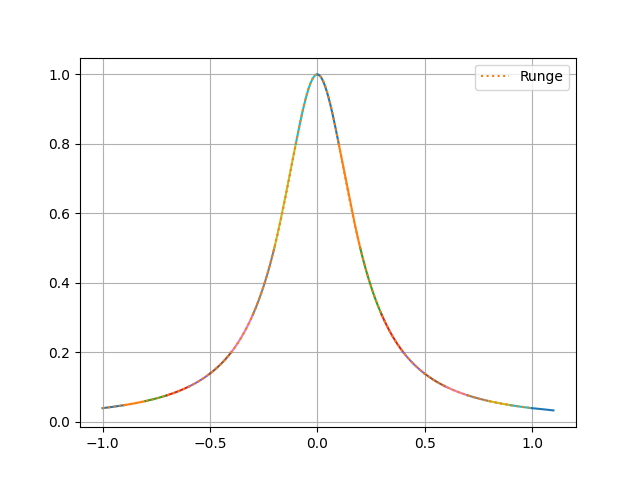
\includegraphics[width=8cm]{SPL.png}
            \caption{SPL内插图像}
        \end{minipage}
        \qquad
        \begin{minipage}{0.45\linewidth}
            \centering
            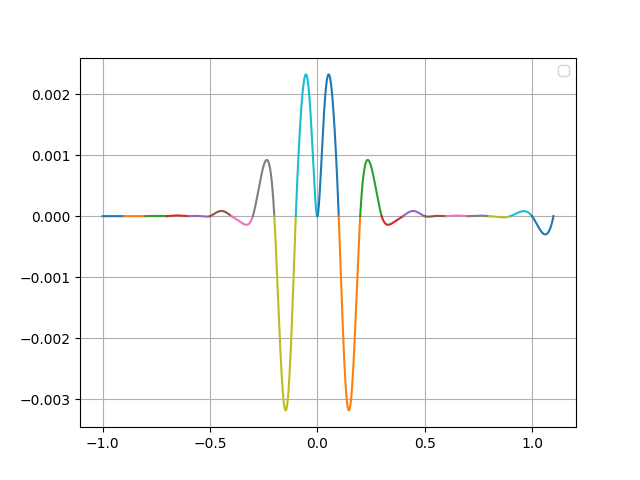
\includegraphics[width=8cm]{errSPL.png}
            \caption{误差$\left [f(x)-SPL(x)\right ]$}
        \end{minipage}
    \end{figure}
    三次样条插值比Chebyshev的稳定性更好,误差振幅更小,而且衰减更快。
\end{answer}
\textbf{5.样条函数在计算机绘图中的运用}\ 本题中我们考虑Cubic\ spline在计算机绘图中的广泛运用。我们将尝试用三次样条函数平滑地连接若干个二维空间中已知的点。
考虑二维空间的一系列点$(x_i, y_i)i=0,1,\cdots,n$。我们现在希望按照顺序(由$0$到$n$)将它们平滑地连接起来。一个方便的办法
是引入一个连续参数$t\in[0,n]$,取节点为$t_i=0,1,\cdots,n$,然后分别建立两个样条函数:$S_{\Delta}(X;t)$和$S_{\Delta}(Y;t)$它们分别满足
$$S_{\Delta}(X;t_i)=x_i,\ S_{\Delta}(Y;t_i)=y_i.$$
这两个样条函数可以看做是$(x(t),y(t))$的内插近似。因此绘制参数曲线$(x(t),y(t))$的问题就化为求出两个样条函数
并将它们画出的问题。我们考虑的函数是著名的心形线(cardioid)。它的极坐标方程是
$$r(\phi)=2a(1-\cos{\phi})=1(1-\cos{\phi}).$$
为了方便起见我们取了$2a=1$。(请利用上一题中关于样条函数内插的相应代码来处理本题)

(a)选取$\phi=t\pi/4,\ t=0,1,2,3,4,5,6,7,8$这九个点,给出$x_t=r(\phi)\cos{\phi}$和$y_t=r(\phi)\sin{\phi}$的数值。
将这些数值作为精确的数值列在一个表里。
\begin{answer}
    可以借助程序得到结果,代码是trivial的,这里不给出了。结果如下。
    \begin{table}[H]
        \centering
        \begin{tabular}{cccccc}
            \toprule
            t & 0 & 1 & 2 & 3 & 4 \\
            \midrule
            $x_t$ & 0.000e+00 & 2.071e-01 & 6.123e-17 & -1.207e+00 & -2.000e+00\\
            $y_t$ & 0.000e+00 & 2.071e-01 & 1.000e+00 & 1.207e+00 & 2.449e-16\\
            \bottomrule
            \toprule
            t & 5 & 6 & 7 & 8 &  \\
            \midrule
            $x_t$ & -1.207e+00 & -1.837e-16 & 2.071e-01 & 0.000e+00 &\\
            $y_t$ & -1.207e+00 & -1.000e+00 & -2.071e-01 & -0.000e+00 &\\
            \bottomrule
        \end{tabular}
        \caption{心形线的几个点的坐标}
    \end{table}
\end{answer}
(b)给出过这8个点的两个三次样条函数$S_{\Delta}(X;t)$和$S_{\Delta}(Y:t)$。
\begin{answer}
    形状依然是
    \begin{align}
        S_{m,m+1}''&=\frac{M_{m+1}(x-x_m)}{x_{m+1}-x_m}+\frac{M_{m}(x_{m+1}-x)}{x_{m+1}-x_m},\notag\\
        S_{m,m+1}'&=\frac{M_{m+1}}{2}\frac{(x-x_m)^2}{x_{m+1}-x_m}-\frac{M_{m}}{2}\frac{(x_{m+1}-x)^2}{x_{m+1}-x_{m}}+A_m,\notag\\
        S_{m,m+1}&=\frac{M_{m+1}}{6}\frac{(x-x_m)^3}{x_{m+1}-x_m}-\frac{M_{m}}{6}\frac{(x-x_{m+1})^3}{x_{m+1}-x_{m}}+A_m(x-x_m)+B_m.\notag
    \end{align}
    借助程序“HW2计物第五题b”给出全部的$M,A,B$,结果如下。
    \begin{table}[H]
        \centering
        \begin{tabular}{cccccc}
            \toprule
            m & 0 & 1 & 2 & 3 & 4 \\
            \midrule
            $ M_{mx}$& -1.077e-01 & -3.457e-01 & -2.539e+00 & 7.730e-01 & 3.476e+00\\
            $ M_{my}$& -4.929e-01 & 1.820e+00 & -1.088e+00 & -3.167e+00 & 4.709e-04\\
            $ A_{mx}$& 2.949e-01 & 2.335e-02 & -1.970e+00 & -1.363e+00 & 1.366e+00\\
            $ A_{my}$& -3.900e-02 & 1.390e+00 & 5.359e-01 & -1.952e+00 & -1.951e+00\\
            $ B_{mx}$& 1.107e-02 & 2.426e-01 & 2.610e-01 & -1.287e+00 & -2.357e+00\\
            $ B_{my}$& 5.067e-02 & 2.004e-02 & 1.112e+00 & 1.533e+00 & -4.842e-05\\
            \bottomrule
            \toprule
            m & 5 & 6 & 7 & 8 & 9\\
            \midrule
            $ M_{mx}$& 7.495e-01 & -2.445e+00 & -6.983e-01 & 1.209e+00 & -1.077e-01\\
            $ M_{my}$& 3.165e+00 & 1.094e+00 & -1.844e+00 & 5.842e-01 & -4.929e-01\\
            $ A_{mx}$&1.955e+00 & 3.512e-02 & -5.133e-01 & 4.360e-01 & \\
            $ A_{my}$&5.348e-01 & 1.394e+00 & -5.417e-02 & 4.047e-01 & \\
            $ B_{mx}$& -1.284e+00 & 2.513e-01 & 2.789e-01 & -1.243e-01 & \\
            $ B_{my}$& -1.533e+00 & -1.112e+00 & -1.752e-02 & -6.006e-02 & \\
            \bottomrule
        \end{tabular}
        \caption{SPL的系数M,A,B}
    \end{table}
\end{answer}
(c)画出参数形式的曲线$(x_t,y_t)=(S_{\Delta}(X;t),S_{\Delta}(Y;t))$,同时画出它所内插的严格的曲线进行比较,请标出相应的节点。
\begin{answer}
    借助程序“HW2计物第五题c”可以作图如下。
    \begin{figure}[H]
        \centering
        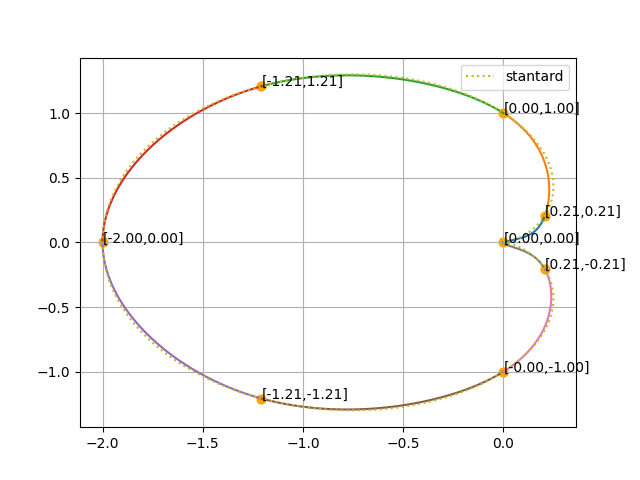
\includegraphics[width=10cm]{cardioid.png}
        \caption{SPL内插心形线}
    \end{figure}
    原函数与相关节点均已标出。可以看出内插效果非常好。
\end{answer}
(d)简要说明为什么这个算法可以平滑地连接所有的点(这实际上是很多画图软件中spline曲线所采用的的算法)。
\begin{answer}
    可以看出来各个节点的连接处,至少到一阶导数都是连续的。由于三次样条内插,一个节点的两端有
    $$S_{\Delta}'(X;k-0)=S_{\Delta}'(X;k+0),\ S_{\Delta}'(Y;k-0)=S_{\Delta}'(Y;k+0).$$
    那么就有
    $$\left(\frac{dS_{\Delta}(X;t)}{dS_{\Delta}(Y;t)}\right)_{t=k-0}=\frac{S_{\Delta}'(X;k-0)}{S_{\Delta}'(Y;k-0)}=\frac{S_{\Delta}'(X;k+0)}{S_{\Delta}'(Y;k+0)}=\left(\frac{dS_{\Delta}(X;t)}{dS_{\Delta}(Y;t)}\right)_{t=k+0}.$$
    一阶导数连续。就很平滑。
\end{answer}
\end{document}